%%%%%%%%%%%%%%%%%%%%%%%%%%%%%%%%%%%%%%%%%
% Structured General Purpose Assignment
% LaTeX Template
%
% This template has been downloaded from:
% http://www.latextemplates.com
%
% Original author:
% Ted Pavlic (http://www.tedpavlic.com)
%
% Note:
% The \lipsum[#] commands throughout this template generate dummy text
% to fill the template out. These commands should all be removed when 
% writing assignment content.
%
%%%%%%%%%%%%%%%%%%%%%%%%%%%%%%%%%%%%%%%%%

%----------------------------------------------------------------------------------------
%	PACKAGES AND OTHER DOCUMENT CONFIGURATIONS
%----------------------------------------------------------------------------------------

\documentclass{article}

\usepackage[UKenglish]{babel}

\usepackage[utf8]{inputenc}
\usepackage{fancyhdr} % Required for custom headers
\usepackage{lastpage} % Required to determine the last page for the footer
\usepackage{extramarks} % Required for headers and footers
\usepackage{graphicx} % Required to insert images
\usepackage{lipsum} % Used for inserting dummy 'Lorem ipsum' text into the template
\usepackage{subfig} % Used for inserting figure side by side
\usepackage{xspace}
\usepackage{hyperref}
\def\code#1{\texttt{#1}}
\newcommand{\MATLAB}{\textsc{Matlab}\xspace}

% Margins
\topmargin=-0.45in
\evensidemargin=0in
\oddsidemargin=0in
\textwidth=6.5in
\textheight=9.0in
\headsep=0.25in 

\linespread{1.1} % Line spacing

% Set up the header and footer
\pagestyle{fancy}
\lhead{\hmwkAuthorName} % Top left header
\rhead{\hmwkClass: \hmwkTitle} % Top center header
\chead{} % Top right header
\lfoot{} % Bottom left footer
\cfoot{} % Bottom center footer
\rfoot{Page\ \thepage\ of\ \pageref{LastPage}} % Bottom right footer
\renewcommand\headrulewidth{0.4pt} % Size of the header rule
\renewcommand\footrulewidth{0.4pt} % Size of the footer rule

\setlength\parindent{0pt} % Removes all indentation from paragraphs

%----------------------------------------------------------------------------------------
%	DOCUMENT STRUCTURE COMMANDS
%	Skip this unless you know what you're doing
%----------------------------------------------------------------------------------------

% Header and footer for when a page split occurs within a problem environment
\newcommand{\enterProblemHeader}[1]{
\nobreak\extramarks{#1}{#1 continued on next page\ldots}\nobreak
\nobreak\extramarks{#1 (continued)}{#1 continued on next page\ldots}\nobreak
}

% Header and footer for when a page split occurs between problem environments
\newcommand{\exitProblemHeader}[1]{
\nobreak\extramarks{#1 (continued)}{#1 continued on next page\ldots}\nobreak
\nobreak\extramarks{#1}{}\nobreak
}

\setcounter{secnumdepth}{0} % Removes default section numbers
\newcounter{homeworkProblemCounter} % Creates a counter to keep track of the number of problems

\newcommand{\homeworkProblemName}{}
\newenvironment{homeworkProblem}[1][Problem \arabic{homeworkProblemCounter}]{ % Makes a new environment called homeworkProblem which takes 1 argument (custom name) but the default is "Problem #"
\stepcounter{homeworkProblemCounter} % Increase counter for number of problems
\renewcommand{\homeworkProblemName}{#1} % Assign \homeworkProblemName the name of the problem
\section{\homeworkProblemName} % Make a section in the document with the custom problem count
\enterProblemHeader{\homeworkProblemName} % Header and footer within the environment
}{
\exitProblemHeader{\homeworkProblemName} % Header and footer after the environment
}

\newenvironment{homeworkSection}[1]{ % New environment for sections within homework problems, takes 1 argument - the name of the section
\renewcommand{\homeworkSectionName}{#1} % Assign \homeworkSectionName to the name of the section from the environment argument
\subsection{\homeworkSectionName} % Make a subsection with the custom name of the subsection
\enterProblemHeader{\homeworkProblemName\ [\homeworkSectionName]} % Header and footer within the environment
}{
\enterProblemHeader{\homeworkProblemName} % Header and footer after the environment
}
   
%----------------------------------------------------------------------------------------
%	NAME AND CLASS SECTION
%----------------------------------------------------------------------------------------

\newcommand{\hmwkTitle}{Coursework 3} % Assignment title
\newcommand{\hmwkClass}{COMP6223 - Computer Vision} % Course/class
\newcommand{\hmwkAuthorName}{Drago Matteo (29824648) \& Azzino Tommy (29824613)} % Your name
\newcommand{\hmwkClassInstructor}{Jonathon Hare} % Teacher/lecturer


%----------------------------------------------------------------------------------------
%	TITLE PAGE
%----------------------------------------------------------------------------------------

\title{
\vspace{2in}
\textmd{\textbf{\hmwkClass \\ \hmwkTitle}}\\
\vspace{3in}
}
\author{\textbf{\hmwkAuthorName}}
\date{} % Insert date here if you want it to appear below your name

%----------------------------------------------------------------------------------------


\begin{document}
\pagenumbering{gobble} % Used to delete the page number on the title page
\maketitle

\clearpage
\pagenumbering{arabic} % Used to reset the page number after the title page
\setcounter{page}{1}

\clearpage
\section{Introduction}
All the code for this coursework has been written in \MATLAB. 

In all our algorithms we used \code{imageDatastore} in order to speed up images retrieval and manipulation. In particular, we decided to use 25\% of the training set for validation: in this way we tested our different algorithms multiple times and in different configuration before categorizing the test set. The split of the training set, where possible, has been done with \code{splitEachLabel}.
\section{Run 1}

As first approach we had to develop a classifier which use as features \textit{tiny images}. This particular representation consists on few simple steps: initially we resize the image to a 16x16 matrix, then we build a vector of 256 pixels composed of the consecutive rows of the new image. 

After that, in order to improve classification performances, we implemented two different types of normalization to the vector, which in the following we refer to as \textbf{x}:
\begin{itemize}
	\item \textbf{standard normalization}: $\mathbf{\bar{x}} = \frac{\mathbf{x} - \mu}{\sigma}$ where $\mu$ is the mean of \textbf{x} and $\sigma$ is its standard deviation
	\item \textbf{unit length normalization}: $\mathbf{\widehat{x}} = \frac{\mathbf{\bar{x}}}{\left \| \mathbf{\bar{x}} \right \|}$
\end{itemize} 
In this way we obtained a set of unit length vectors of zero mean.

The idea behind the classifier is that one vector representing an image of a specific class will likely be similar to other vectors of the same category. So, once we perform this operation for all the training set, we can determine the category of each image of the validation set using the \textbf{k-nearest-neighbour} classifier: this means that we evaluate the distance between the tiny image to validate and all the vectors from the training set; then, we pick the k nearest vectors (of which we know the class) and we classify our image with the most represented class in the neighbourhood. In case we have two classes most represented we can implement different choice polices, in our case we used the first classes returned by MATLAB.

In order to find better performances, we tried to tune the value of k for the several measures of distance available in \code{vl\_alldist2}, in particular:

\begin{equation}
	\mathbf{L_{INF}}=  max|X - Y| \qquad
	\mathbf{L_2}= sum(X - Y)^2 \qquad
	\mathbf{L_1}= sum|X - Y|
\end{equation} 
\begin{figure}[h]
	\centering
		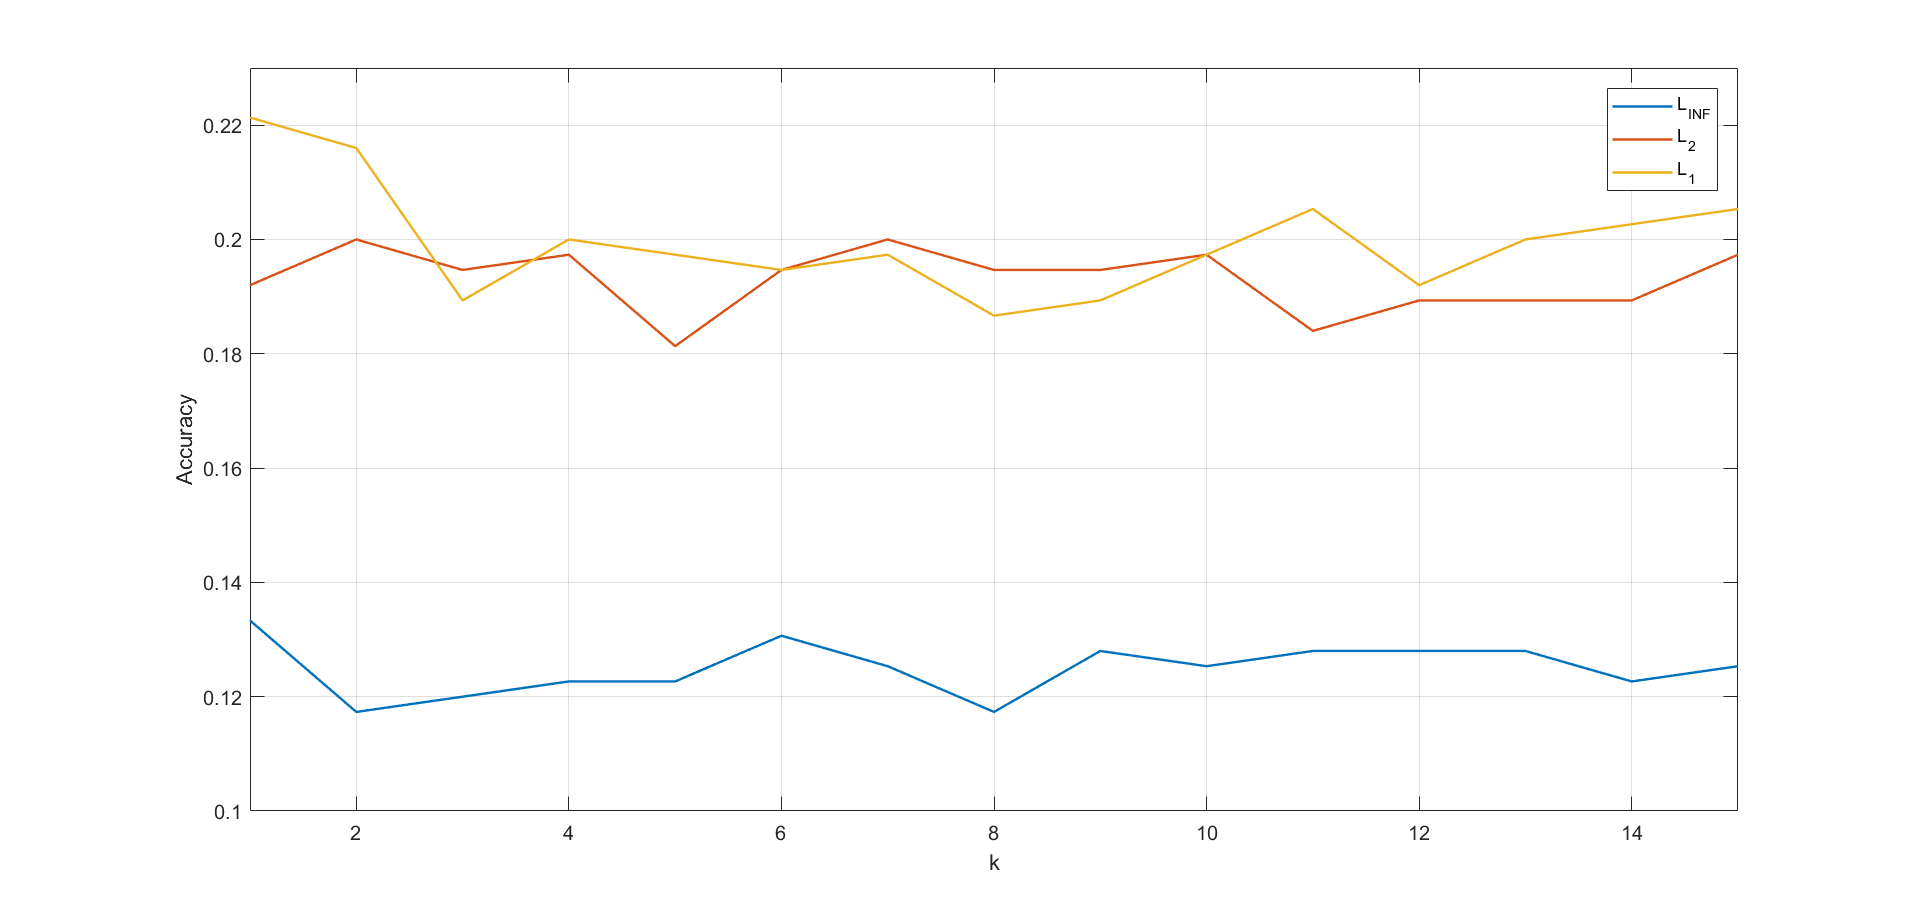
\includegraphics[height=.35\linewidth]{img/kaccuracy}
	\caption{Performances of different distance measures in function of k }
	\label{fig_kaccuracy}
\end{figure}

As we can see from Figure \ref{fig_kaccuracy}, while $L_{INF}$ can't reach even the 14\% of accuracy, $L_2$ and $L_1$ can reach up to 20\% and beyond. It's interesting to highlight that the latter perform better when we use either just the nearest neighbour or we increase the number of neighbours beyond 10, while $L_2$ presents its maximum around 7 or 8.
In conclusion, considering its stable behaviour on different runs that we performed, we decided to implement our classification using $L_2$ with k = 7. Of course, given the simplicity of these features, we couldn't expect more than 20\% of accuracy. On the following sections we will implement different features extraction methods to improve these performances.
\section{run2}

For the run $2$ of the coursework, the objective is to develop a set of linear classifiers for the classification of our test set images. 
\section{Run 3}
For this last approach we decided to implement \textbf{transfer learning}: this means that in order to extract significant features from our images we used layers of a pre-trained neural network. So, to complete our classification architecture, we re-trained just the last layers used for classification on our training set, without doing backpropagation on the previous layers. Surely one advantage of this solution is that allowed us to save a considerable amount of computational time for the training of all the layers of the network.

For this particular problem we decided to use the convolutional neural network (CNN) \code{alexnet}, winner of the 2012 ImageNet Large Scale Visual Recognition Challenge (ILSVRC2012). At the time, it takes an entire week to train the complete network with the competition dataset (1.2M of images).

The main difference with respect to standard NN is that in CNNs neurons are arranged in three spatial dimensions, and so they take 3D inputs and return 3D outputs. This is the main peculiarity that allows CNN performing so good and being so fast: we can clearly see the advantage if we have manipulate RGB images, which have 3 different layers (\textit{Red, Green} and \textit{Blue}), instead of grayscale ones. 

Delving more into some details of \code{alexnet}, we can subdivide its layers in the following types:
\begin{itemize}
	\item INPUT: it accepts 227x227x3 images, so we wrote \code{preprocessingFcn} to resize the images when importing them from the datastore.
	\item CONVOLUTIONAL: it consists of a set of 3D convolutional filters used to actually extract features from the image; each different convolutional layer in the network extracts a set of different features, depending on the characteristics of the filter.
	\item ReLU: it applies the $max(0,x)$ \textbf{activation function} to the output of the convolutional layer; these types of layer in particular are involved in backpropagation, when the network is initially trained.
	\item POOL: it performs downsampling (useful when the work has to be split between two different workers, as during the training of \code{alexnet})
	\item FC (fully connected): refined features comes out from this layer.
\end{itemize}

In our case, we chopped off the network on the $20^{th}$ layer; so, we use features extracted from layer \code{fc7}. All the code of this part can be found in \code{featuresExtractionNetwork}. 

After that, we used the features from the training set to train our classifier. Specifically we used an error-correcting output codes (ECOC) classifier, particularly good when it comes to multiclass learning: it proceeds by reducing the problem to multiple binary classifiers (thanks to coding strategies) such as Support Vector Machines (which we used in our configuration). 

We tested different coding designs (which determine the policy used to reduce the structure to binary learners) on the validation set, obtaining the accuracy values listed in Table 1. Of course the more complex is one strategies, more time it takes to train the classifier. 

\begin{table}[h]
	\centering
	\begin{tabular}{|c|c|c|}
		\hline
		\textbf{Coding Strategy}  & \textbf{Accuracy} \\ \hline
		One VS All & 0.8427           \\ \hline
		One VS One & 0.8400 \\ \hline
		Ordinal & 0.6960 \\ \hline
		Sparse Random & 0.8283 \\ \hline
	\end{tabular}
	\caption{Accuracy with different coding strategies}
	\label{tab:MSE}
\end{table}

We found our best results using \code{onevsall} and we decided to implement it also with our final predictions; looking to the confusion matrix in Figure \ref{fig:heat} we can notice more in detail errors made from the classifier. For example, \textit{Coast} has been misclassified twice with \textit{OpenCountry} while \textit{Bedroom} has been mostly misclassified with \textit{LivingRoom}. This suggests us that our architectureis vulnerable when dealing with images that could have really similar features.  

\begin{figure}[!htbp] 
	\centering
	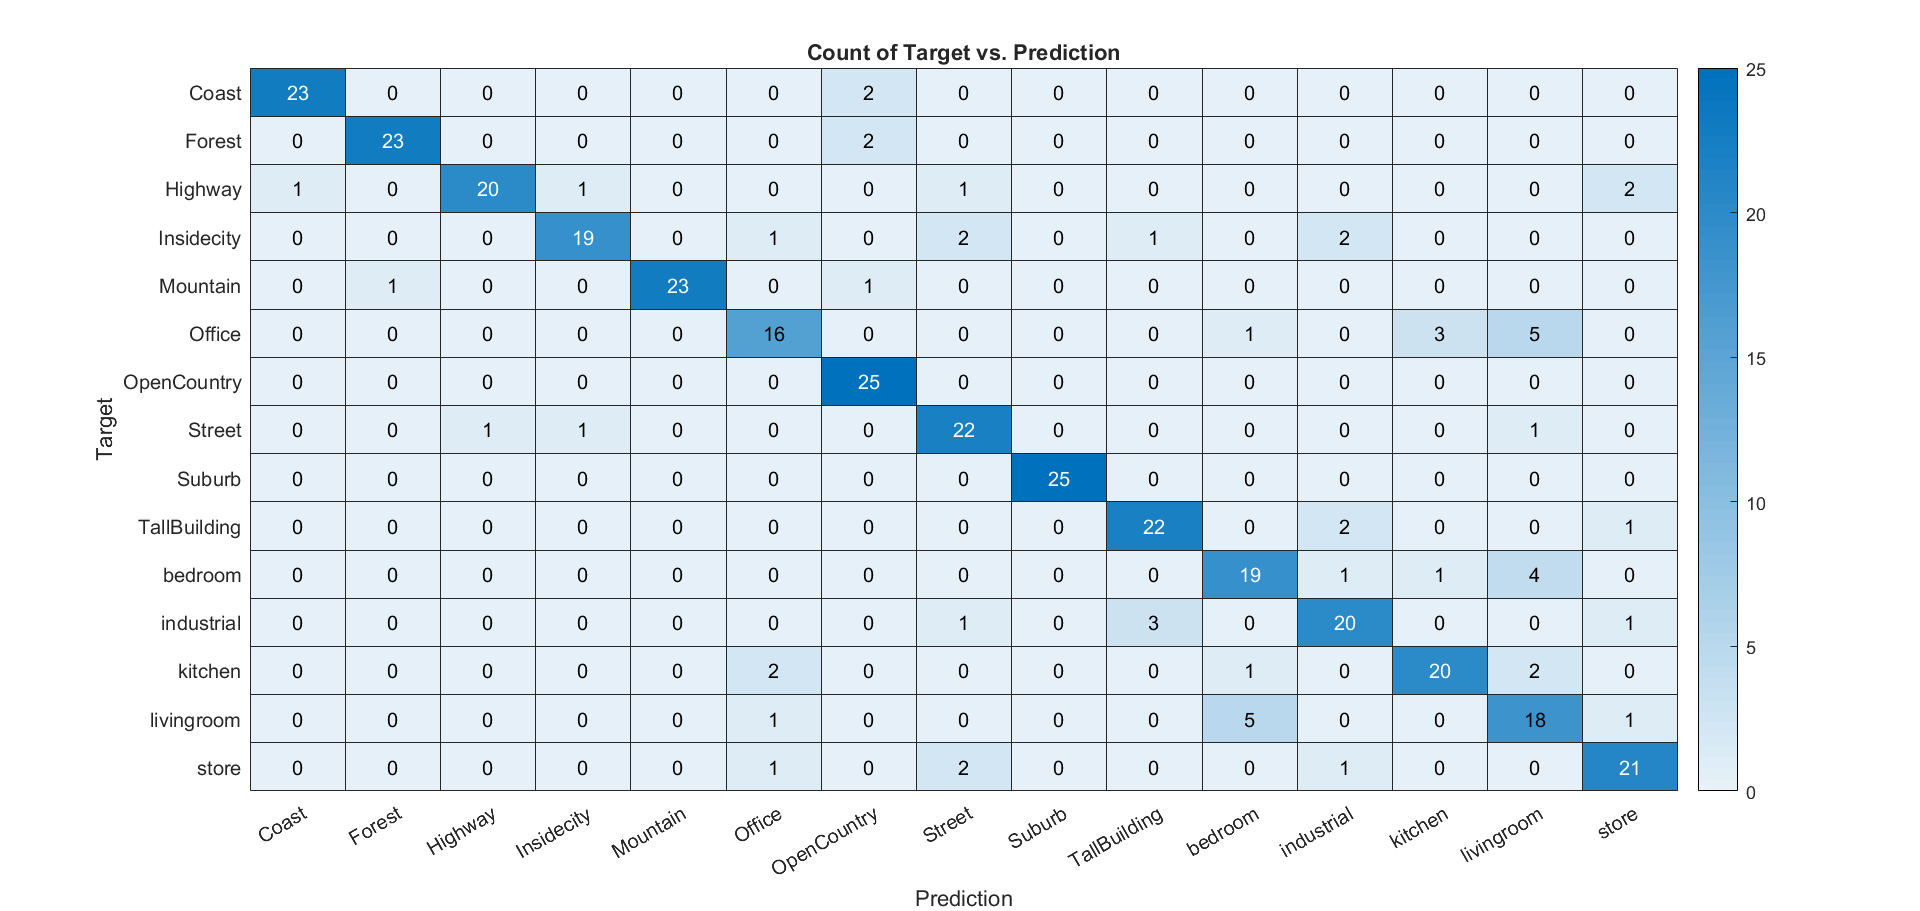
\includegraphics[width=1\linewidth]{img/heatmap}
	\caption{Confusion matrix obtained with one-vs-all coding design}
	\label{fig:heat}
\end{figure}
\section{References}

[1] \href{http://www.vlfeat.org/matlab/matlab.html}{http://www.vlfeat.org/matlab/matlab.html}


\section{Contributions statement}

Each member of the group has contributed in equal manner during the code development of the $3$ runs and writing of the report. Also considerations regarding each run have been conducted together. 


\end{document}